Serieschaltung von Widerstand und Kondensator an einem Rechtecksignal $U_e$\\
\begin{tabular}{ccc}
	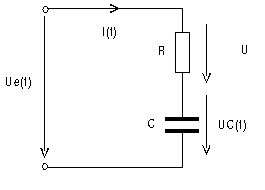
\includegraphics[width=3.5cm]{./idiotenseite/images/schaltung_C.png} &
	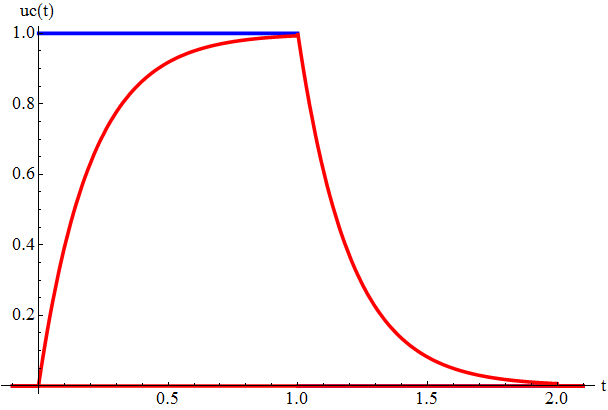
\includegraphics[width=3.5cm]{./idiotenseite/images/uKond.png} &
	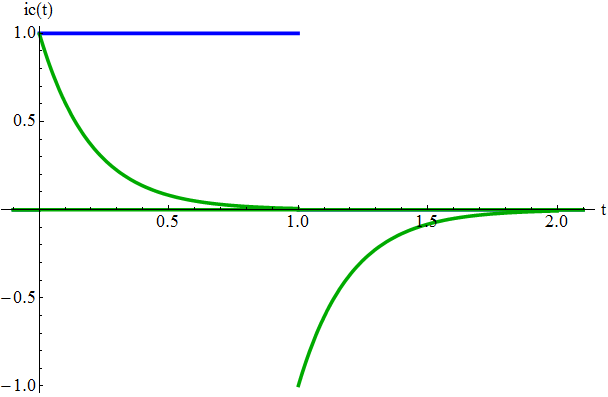
\includegraphics[width=3.5cm]{./idiotenseite/images/iKond.png}\\
\end{tabular}
\begin{multicols}{2}		
	Ladevorgang:\\
	$u_{\mathrm{C}} (t) = U_0 \cdot \biggl(1 - e^{- \frac{t}{\tau}}\biggr) = U_0
	\cdot \biggl(1 - e^{- \frac{t}{R_{\mathrm{C}} \cdot C}}\biggr)$\\
	$i_{\mathrm{C}} (t) = \frac{U_0}{R_{\mathrm{C}}} \cdot e^{- \frac{t}{\tau}} =
	I_0 \cdot e^{- \frac{t}{R_{\mathrm{C}} \cdot C}}$\\
	\newline
	Entladevorgang\\
	$u_{\mathrm{C}} (t) = U_0 \cdot e^{- \frac{t}{\tau}} = U_0 \cdot e^{-
	\frac{t}{R_{\mathrm{C}} \cdot C}}$\\
	$i_{\mathrm{C}} (t) = -	\frac{U_0}{R_{\mathrm{C}}} \cdot e^{- \frac{t}{\tau}}
	= - I_0 \cdot e^{-\frac{t}{R_{\mathrm{C}} \cdot C}}$\\
\end{multicols}

